\documentclass{standalone}
% fonts
\usepackage{mathpazo} % math & rm
\linespread{1.05} % Palatino needs more leading (space between lines)
% tikz
\usepackage{tikz}
\usetikzlibrary{positioning,shapes}
\begin{document}
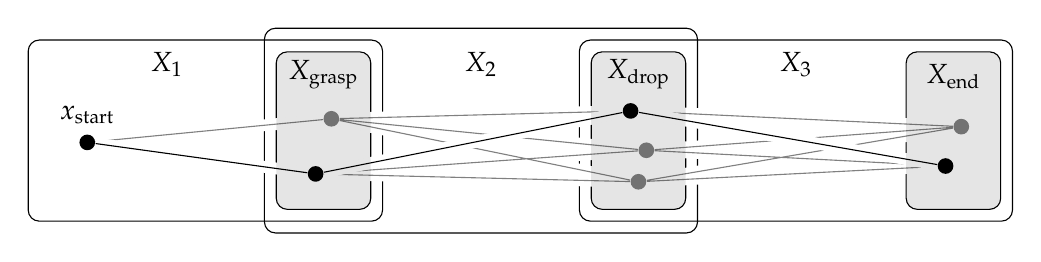
\begin{tikzpicture}
\tikzset{>=latex} % arrow heads

% middle: c-space sequence
% valid subsets
\node[draw,black,rounded corners,
   minimum height=2.3cm,minimum width=4.5cm]
   (X1) at (-3.5,-4.75) {};
\node[draw,black,rounded corners,
   minimum height=2.6cm,minimum width=5.5cm]
   (X2) at (0,-4.75) {};
\node[draw,black,rounded corners,
   minimum height=2.3cm,minimum width=5.5cm]
   (X3) at ( 4,-4.75) {};
% root sets
\node[draw,black,rounded corners,
   minimum height=2cm,minimum width=1.2cm]
   (Xgrasp) at (-2,-4.75) {};
\node[draw,black,rounded corners,
   minimum height=2cm,minimum width=1.2cm]
   (Xdrop) at (2,-4.75) {};
\node[draw,black,rounded corners,
   minimum height=2cm,minimum width=1.2cm]
   (Xend) at (6,-4.75) {};
% set labels
\node[above=-0.6cm of Xgrasp] {$X_{\mbox{\scriptsize grasp}}$};
\node[above=-0.6cm of Xdrop] {$X_{\mbox{\scriptsize drop}}$};
\node[above=-0.6cm of Xend] {$X_{\mbox{\scriptsize end}}$};
\node[above left=-0.6cm and -2.1cm of X1] {$X_1$};
\node[above=-0.75cm of X2] {$X_2$};
\node[above=-0.6cm of X3] {$X_3$};
% nodes and paths
\node[circle,fill=black,inner sep=2] (xstart) at (-5,-4.9) {};
\node[circle,fill=black!50,inner sep=2] (xg1) at (-1.9,-4.6) {};
\node[circle,fill=black,inner sep=2] (xg2) at (-2.1,-5.3) {};
\node[circle,fill=black,inner sep=2] (xd1) at ( 1.9,-4.5) {};
\node[circle,fill=black!50,inner sep=2] (xd2) at ( 2.1,-5.0) {};
\node[circle,fill=black!50,inner sep=2] (xd3) at ( 2.0,-5.4) {};
\node[circle,fill=black!50,inner sep=2] (xe1) at ( 6.1,-4.7) {};
\node[circle,fill=black,inner sep=2] (xe2) at ( 5.9,-5.2) {};
\node[above=0cm of xstart] {$x_{\mbox{\scriptsize start}}$};
% lines
\draw[line width=1.5mm,white]
   (xstart) -- (xg1) (xg1) -- (xd1) (xg1) -- (xd2) (xg1) -- (xd3)
   (xg2) -- (xd2) (xg2) -- (xd3) (xd1) -- (xe1) (xd2) -- (xe1)
   (xd2) -- (xe2) (xd3) -- (xe1) (xd3) -- (xe2);
\draw[draw=black!50]
   (xstart) -- (xg1) (xg1) -- (xd1) (xg1) -- (xd2) (xg1) -- (xd3)
   (xg2) -- (xd2) (xg2) -- (xd3) (xd1) -- (xe1) (xd2) -- (xe1)
   (xd2) -- (xe2) (xd3) -- (xe1) (xd3) -- (xe2);
\draw[line width=1.5mm,white]
   (xstart) -- (xg2) (xg2) -- (xd1) (xd1) -- (xe2);
\draw
   (xstart) -- (xg2) (xg2) -- (xd1) (xd1) -- (xe2);
% grey sets (overlay)
\node[fill=black,opacity=0.1,rounded corners,
   minimum height=2cm,minimum width=1.2cm]
   at (-2,-4.75) {};
\node[fill=black,opacity=0.1,rounded corners,
   minimum height=2cm,minimum width=1.2cm]
   at (2,-4.75) {};
\node[fill=black,opacity=0.1,rounded corners,
   minimum height=2cm,minimum width=1.2cm]
   at (6,-4.75) {};

\end{tikzpicture}%
\end{document}
